\chapter{Results and Discussion}
\label{chap:results}

\chapterintro{%
This chapter reports software, RTL, post-route, and physical-board results in their
respective evidence categories. The central result is a same-board comparison of
five independent fixed-point candidate-evaluation configurations.}

\section{Experimental Overview}

The evaluation followed four linked stages. Offline software training and held-out
traces established controller behavior. Exhaustive and integrated RTL tests checked
state encoding, policy lookup, dwell control, fixed-point arithmetic, and protocol
timing. Independent Xilinx ISE builds provided post-route timing and resource data.
Finally, the same Nexys 3 board replayed a common physical corpus for all five
configurations.

The strongest comparison is internal Class A evidence: identical board, shell,
clock, widths, record schema, and measurement boundary. Route-quality statistics
are reported separately from exactness and implementation metrics.

\section{Offline Controller Behavior}

Each of the eight policy candidates completed 819,200 training transitions. Seven
passed the validation criteria, and seed 229 was selected by the declared ranking.
Table~\ref{tab:heldout-software} summarizes the four-trace held-out software
partition after the policy was fixed. All controllers completed 2,048 successful
decisions with zero blocking in this controlled environment.

\begin{table}[H]
\centering
\caption{Software-simulated held-out controller behavior over four
512-decision traces.}
\label{tab:heldout-software}
\begin{tabularx}{\textwidth}{@{}p{0.28\textwidth}rrrrrr@{}}
\toprule
\textbf{Controller} & \makecell{\textbf{Mean}\\\textbf{evaluation}\\\textbf{reward}} &
\textbf{Block} & \textbf{Quality} &
\makecell{\textbf{Mean}\\\textbf{balance}\\\textbf{utility}} & \textbf{Hops} &
\textbf{Switch rate}\\
\midrule
Fixed-profile & 4.6130 & 0 & 0.95815 & 0.16881 & 2.8750 & 0\\
Rule-adaptive & 4.6292 & 0 & 0.95943 & 0.25513 & 2.9775 & 0.2813\\
Offline-learned adaptive & 4.6771 & 0 & 0.96044 & 0.26499 & 2.9541 & 0.2329\\
\bottomrule
\end{tabularx}
\end{table}

All reward values in Table~\ref{tab:heldout-software} are means of
$r_t^{\mathrm{eval}}$. The learned policy had the highest descriptive mean
evaluation reward and the highest reported mean balance utility in this software
partition. Because $U_B=1-\operatorname{clip}_{[0,1]}(I_t^{\rm post})$, larger
balance utility means lower post-decision imbalance under the defined utility.
With only four paired traces, the exact two-sided
permutation $p$-value was 0.125 and the Holm-adjusted value was 0.25 for both learned
comparisons. The software result therefore describes behavior under the selected
environment; it is not evidence of statistical superiority.

The learned mean of 4.677079 is an evaluation-scale mean of
$r_t^{\mathrm{eval}}$, not a training-target mean. It is interpreted using
Equations~\eqref{eq:success-reward}--\eqref{eq:block-reward}. Zero blocking means
each step received the $+4$ success term. The remaining approximately 0.677 mean
contribution is the net of bounded route-quality and balance utilities, hop costs,
and profile-switch penalties. It is not an end-to-end secret-key rate, monetary
value, or physical energy measure. The route-quality column likewise reports the
registered synthetic metric; it is not evidence of coherence in a stored classical
key pool.

\section{Controller and Policy Verification}

\begin{table}[H]
\centering
\caption{Controller and policy verification summary.}
\label{tab:controller-verification}
\begin{tabularx}{\textwidth}{@{}X r X@{}}
\toprule
\textbf{Verification item} & \textbf{Count/result} & \textbf{Outcome}\\
\midrule
Encoded state addresses & 256/256 & Exact policy/state mapping\\
Threshold below/equal/above cases & 36 & Equality entered the higher bin\\
Profile actions & 4/4 & All profiles covered\\
Cycle vectors & 1,509 & Zero RTL mismatch\\
Valid decisions & 302 & Zero unexplained mismatch\\
Python regression tests & 74 & Pass\\
Lint warnings & 0 & Pass\\
Controller-only synthesis estimate & 103 LUTs, 79 registers & Synthesis pass\\
\bottomrule
\end{tabularx}
\end{table}

The controller-only synthesis reported an estimated maximum frequency of
247.812~MHz. This value is a post-synthesis estimate for the isolated controller and
is not used as the system frequency. Final maximum-frequency results are taken from
complete post-route implementations.

\section{Integrated RTL Verification}

Integrated cycle-accurate tracing added 2,125 cycle vectors and 530 valid decisions.
The valid-request controller path had a deterministic three-cycle latency. Reset,
busy, no-path, invalid-input, threshold equality, dwell hold, dwell switch, and
pipeline-wait cases were exercised. Candidate-evaluator regression covered 519 of
519 vectors, and the integrated policy shell matched 101 of 101 expected results.
These are RTL-simulated results; physical exactness is established by the board
replay below.

\section{Independent FPGA Implementation}

Configurations H0--H4 were built independently for the XC6SLX16-2-CSG324 device.
Each build passed synthesis, mapping, placement, routing, and the 100~MHz timing
constraint. Independent bitstreams prevent a parameter-only simulation from being
reported as multiple physical implementations. Configuration H0 remained the
feasible minimum-hop baseline, while configurations H1--H4 added the
cost and profile-scoring functions defined in
Table~\ref{tab:h0-h4-definitions}.

\section{Same-Board Physical Replay and Exactness}

Each configuration produced 84 physical records: 20 directed contract records and
64 held-out records. Nine output fields were checked per record. Table
\ref{tab:physical-exactness} reports the exact comparison.

\begin{table}[H]
\centering
\caption{Physical replay exactness for the five independent configurations.}
\label{tab:physical-exactness}
\begin{tabular}{@{}lrrrr@{}}
\toprule
\textbf{Configuration} & \textbf{Records} & \textbf{Fields/record} &
\textbf{Exact fields} & \textbf{Mismatches}\\
\midrule
H0 & 84 & 9 & 756 & 0\\
H1 & 84 & 9 & 756 & 0\\
H2 & 84 & 9 & 756 & 0\\
H3 & 84 & 9 & 756 & 0\\
H4 & 84 & 9 & 756 & 0\\
\midrule
\textbf{Total} & \textbf{420} & --- & \textbf{3,780} & \textbf{0}\\
\bottomrule
\end{tabular}
\end{table}

This result establishes that physical transport and parsing functioned, each
independent implementation matched its fixed-point contract, and configuration H4
performed policy/profile inference consistently with the reference. Exactness does
not by itself establish that one controller selects higher-quality routes.

\section{Post-Route Timing and Kernel Latency}

\begin{table}[H]
\centering
\caption{Post-route maximum frequency and measured kernel latency under the common
100~MHz operating contract.}
\label{tab:same-board-timing}
\small
\begin{tabularx}{\textwidth}{@{}lXrrr@{}}
\toprule
\textbf{Configuration} & \textbf{Selection method} &
\textbf{$f_{\max}$ (MHz)} & \textbf{Mean cycles} &
\textbf{Latency ($\mu$s)}\\
\midrule
H0 & Feasible minimum-hop baseline & 118.948 & 2.000 & 0.020\\
H1 & Fixed key-aware baseline & 107.538 & 201.763 & 2.018\\
H2 & Fixed-profile \QFlow & 102.838 & 202.763 & 2.028\\
H3 & Threshold/rule adaptive & 102.648 & 202.763 & 2.028\\
H4 & Reinforcement-learned adaptive & 102.020 & 204.763 & 2.048\\
\bottomrule
\end{tabularx}
\end{table}

All configurations exceeded 100~MHz. Configuration H4 achieved a post-route maximum
frequency of 102.020~MHz and a mean normal-case latency of 2.047632~$\mu$s, rounded
to 2.048~$\mu$s. This is the accepted-request-to-done latency of the tested FPGA
kernel. UART serialization, host processing, KMS acquisition, candidate generation,
security checks, and route installation are outside the measurement.

\begin{figure}[H]
\centering
\begin{subfigure}[t]{0.49\textwidth}
\centering
\begin{tikzpicture}
\begin{axis}[
  ybar,width=\textwidth,height=6.0cm,ymin=95,ymax=122,
  ylabel={$f_{\max}$ (MHz)},symbolic x coords={H0,H1,H2,H3,H4},xtick=data,
  bar width=12pt,nodes near coords,grid=major,grid style={QFlowLine!45},
  tick label style={font=\scriptsize},label style={font=\scriptsize},
  every node near coord/.append style={font=\tiny}]
\addplot[fill=QFlowBlue!75,draw=QFlowBlue] coordinates
{(H0,118.948)(H1,107.538)(H2,102.838)(H3,102.648)(H4,102.020)};
\end{axis}
\end{tikzpicture}
\caption{Post-route maximum frequency.}
\end{subfigure}\hfill
\begin{subfigure}[t]{0.49\textwidth}
\centering
\begin{tikzpicture}
\begin{axis}[
  ybar,width=\textwidth,height=6.0cm,ymin=0,ymax=2.25,
  ylabel={Kernel latency ($\mu$s)},symbolic x coords={H0,H1,H2,H3,H4},xtick=data,
  bar width=12pt,nodes near coords,grid=major,grid style={QFlowLine!45},
  tick label style={font=\scriptsize},label style={font=\scriptsize},
  every node near coord/.append style={font=\tiny}]
\addplot[fill=QFlowTeal!75,draw=QFlowTeal] coordinates
{(H0,0.020)(H1,2.018)(H2,2.028)(H3,2.028)(H4,2.048)};
\end{axis}
\end{tikzpicture}
\caption{Mean normal-case latency.}
\end{subfigure}
\caption{Timing and latency across the H0--H4 comparison.}
\label{fig:timing-latency}
\end{figure}

The reciprocal of the rounded configuration H4 kernel latency is
$1/(2.048~\mu\mathrm{s})\approx488{,}281$ transactions/s. This is a theoretical
sequential kernel-service rate under immediate back-to-back acceptance, not measured
end-to-end throughput.

Configuration H0 is not feature-equivalent to the remaining configurations; its
two-cycle result should not be used to calculate an RL overhead. The relevant
adaptive comparison is configuration H4 versus configuration H3.

The timing separation follows directly from the implemented datapaths. H0 selects
the valid candidate with the smallest hop count, using candidate slot as the
deterministic tie-break, and registers completion without range normalization.
H1--H4 use the shared iterative 49-by-33-bit divider; objective ranges that are not
equal require repeated division steps, so their median is near the 309--312-cycle
maximum even though bypassed cases reduce the mean. H1 omits the profile-ROM read.
H2 and H3 add that one setup cycle, and their common candidate evaluator therefore
has the same measured mean. H4 adds two controller cycles for policy-ROM/dwell
inference and retains the same scoring engine. The resulting H4--H3 difference is
two cycles, or 20~ns at 100~MHz, while the full H0--H4 gap mainly measures the
presence of the multi-objective evaluator rather than reinforcement learning.

\section{Resource Utilization}

\begin{table}[H]
\centering
\caption{Post-route resource utilization of independent H0--H4 implementations.}
\label{tab:resources}
\begin{tabular}{@{}lrrr@{}}
\toprule
\textbf{Configuration} & \textbf{Slice registers} & \textbf{Slice LUTs} &
\textbf{Occupied slices}\\
\midrule
H0 & 493 & 801 & 301\\
H1 & 1,000 & 1,484 & 589\\
H2 & 1,085 & 1,650 & 649\\
H3 & 1,097 & 1,836 & 645\\
H4 & 1,156 & 1,706 & 677\\
\bottomrule
\end{tabular}
\end{table}

Configuration H4 used 1,706 LUTs, 1,156 registers, and 677 occupied slices. Relative
to configuration H3, it mapped to 7.081\% fewer LUTs, 5.378\% more registers, and
4.961\% more occupied slices. LUT count and occupied slices can move in opposite
directions because slice packing, register placement, and routing affect physical
occupancy. The LUT reduction is an implementation-specific synthesis result, not a
general property of reinforcement learning.
Figure~\ref{fig:resource_utilization} plots the three resource categories on
separate zero-based axes, making the H3--H4 mapping trade-off visible without
combining unlike resources on one scale.

\begin{table}[H]
\centering
\caption{Detailed H4 utilization from the Xilinx map report for
XC6SLX16-2-CSG324. Percentages are the report's integer values.}
\label{tab:h4-device-utilization}
\begin{tabularx}{\textwidth}{@{}X r r r@{}}
\toprule
\textbf{Resource} & \textbf{Used} & \textbf{Available} & \textbf{Utilization}\\
\midrule
Slice registers & 1,156 & 18,224 & 6\%\\
Slice LUTs & 1,706 & 9,112 & 18\%\\
Occupied slices & 677 & 2,278 & 29\%\\
Bonded I/O blocks & 17 & 232 & 7\%\\
RAMB16 block RAMs & 0 & 32 & 0\%\\
RAMB8 block RAMs & 0 & 64 & 0\%\\
BUFG global clock buffers & 1 & 16 & 6\%\\
DSP48A1 slices & 0 & 32 & 0\%\\
\bottomrule
\end{tabularx}
\end{table}

The zero BRAM and DSP counts in Table~\ref{tab:h4-device-utilization} are explicit
tool-report entries, not assumptions from missing categories. Policy and profile
storage mapped into distributed logic for this small design. Occupied-slice
capacity also explains why 677 slices correspond to the report's 29\% even though
individual LUT and register percentages are lower.

\section{Adaptive Profile Behavior}

\begin{table}[H]
\centering
\caption{Profile use and switching over 81 valid adaptive decisions.}
\label{tab:adaptation}
\begin{tabular}{@{}lrrrrrrrr@{}}
\toprule
& \multicolumn{4}{c}{\textbf{Profile count}} &
\textbf{Transitions} & \textbf{Runs} & \textbf{Min dwell} & \textbf{Max dwell}\\
\cmidrule(lr){2-5}
\textbf{Configuration} & $\Pi_0$ & $\Pi_1$ & $\Pi_2$ & $\Pi_3$ & & & &\\
\midrule
H3 & 24 & 36 & 18 & 3 & 44 & 45 & 1 & 7\\
H4 & 42 & 11 & 18 & 10 & 24 & 25 & 1 & 7\\
\bottomrule
\end{tabular}
\end{table}

\begin{figure}[H]
\centering
\begin{subfigure}[t]{0.58\textwidth}
\centering
\begin{tikzpicture}
\begin{axis}[
  ybar stacked,width=\textwidth,height=6.1cm,ymin=0,ymax=90,
  ylabel={Valid decisions},symbolic x coords={H3,H4},xtick=data,bar width=28pt,
  legend style={at={(0.5,-0.18)},anchor=north,legend columns=4,font=\scriptsize},
  grid=major,grid style={QFlowLine!45},tick label style={font=\small},
  label style={font=\small}]
\addplot[fill=QFlowBlue!80] coordinates {(H3,24)(H4,42)};
\addplot[fill=QFlowTeal!80] coordinates {(H3,36)(H4,11)};
\addplot[fill=QFlowAmber!80] coordinates {(H3,18)(H4,18)};
\addplot[fill=QFlowGreen!80] coordinates {(H3,3)(H4,10)};
\legend{$\Pi_0$,$\Pi_1$,$\Pi_2$,$\Pi_3$}
\end{axis}
\end{tikzpicture}
\caption{Profile distribution.}
\end{subfigure}\hfill
\begin{subfigure}[t]{0.38\textwidth}
\centering
\begin{tikzpicture}
\begin{axis}[
  ybar,width=\textwidth,height=6.1cm,ymin=0,ymax=50,ylabel={Transitions},
  symbolic x coords={H3,H4},xtick=data,bar width=24pt,nodes near coords,
  grid=major,grid style={QFlowLine!45},tick label style={font=\small},
  label style={font=\small}]
\addplot[fill=QFlowRed!70,draw=QFlowRed] coordinates {(H3,44)(H4,24)};
\end{axis}
\end{tikzpicture}
\caption{Profile transitions.}
\end{subfigure}
\caption{Trace-specific adaptive behavior of configurations H3 and H4.}
\label{fig:adaptation}
\end{figure}

The complete configuration H4 controller, including the offline-learned policy ROM
and minimum-dwell mechanism, reduced observed profile transitions from 44 to 24.
This is a 45.455\% reduction on the evaluated replay, while mean dwell increased
from 1.80 to 3.24 valid decisions. Isolating the learned policy contribution would
require a policy-by-dwell ablation.

The denominator 81 is the number of protocol-valid adaptive decisions in the full
84-row corpus. Records with test IDs 4, 1015, and 1047 were deliberately malformed
and returned \texttt{INVALID\_REQUEST}; they were excluded because no valid
controller decision occurred. The five \texttt{NO\_PATH} records (IDs 3, 1007,
1023, 1039, and 1055) remained included: they carried valid state inputs, advanced
the profile/dwell controller, and failed only because no candidate was feasible.
Thus the profile counts sum to 81 for both H3 and H4.

\section{Held-Out Route-Quality Analysis}

All configurations had 58 successful, four no-path, and two invalid rows in the
64-row held-out physical partition. Upstream candidate validity and the common
request fields determine those outcomes before profile-conditioned soft preference;
the FPGA gates supplied validity rather than recomputing link eligibility.
Consequently, a mode could not convert a deliberately invalid row into
a valid request or select a route when both candidates were infeasible. Differences
appeared only in which feasible candidate was preferred. Table
\ref{tab:pairwise-quality} therefore compares configuration H4 with H2 and H3 only
on the 58 jointly successful rows.

\begin{table}[H]
\centering
\caption{Paired held-out physical route-quality comparisons.}
\label{tab:pairwise-quality}
\begin{tabularx}{\textwidth}{@{}lrrrrrr@{}}
\toprule
\textbf{Comparison} & \textbf{Pairs} & \textbf{Mean diff.} &
\textbf{95\% CI} & \textbf{$p$} & \textbf{$d_z$} & \textbf{Path changes}\\
\midrule
H4--H2 & 58 & 86.47 & $[-25.12,226.62]$ & 0.2188 & 0.176 & 6\\
H4--H3 & 58 & $-78.05$ & $[-242.28,77.53]$ & 0.4531 & $-0.127$ & 7\\
\bottomrule
\end{tabularx}
\end{table}

The route-quality field is unsigned UNORM16: valid codes are 0--65,535, larger is
better, and one unit is $1/65535\approx0.000015259$ of full scale. The exact mean
H4--H2 difference of $+86.465517$ units equals $+0.00131938$ normalized, or about
$+0.132$ percentage points of full scale. The H4--H3 difference of $-78.051724$
units equals $-0.00119099$, or about $-0.119$ percentage points. These effects are
small relative to the complete scale. In H4--H2, 5 pairs were higher, 1 lower, and
52 tied; in H4--H3, 2 were higher, 5 lower, and 51 tied.

\begin{figure}[H]
\centering
\begin{tikzpicture}
\begin{axis}[
  width=0.82\textwidth,height=6.2cm,xmin=-300,xmax=300,ymin=0.5,ymax=2.5,
  xlabel={Mean paired difference (UNORM16 route-quality units)},
  ytick={1,2},yticklabels={H4--H3,H4--H2},
  grid=major,grid style={QFlowLine!45},tick label style={font=\small},
  label style={font=\small}]
\addplot[QFlowGray,dashed,thick] coordinates {(0,0.5)(0,2.5)};
\addplot[QFlowTeal,very thick] coordinates {(-242.28,1)(77.53,1)};
\addplot[QFlowBlue,very thick] coordinates {(-25.12,2)(226.62,2)};
\addplot[only marks,mark=*,mark size=3pt,QFlowTeal] coordinates {(-78.05,1)};
\addplot[only marks,mark=*,mark size=3pt,QFlowBlue] coordinates {(86.47,2)};
\end{axis}
\end{tikzpicture}
\caption{Paired mean route-quality differences with 10,000-replicate paired-row
percentile 95\% confidence intervals (seed 20260731). Both intervals cross zero;
the line at zero denotes no mean difference.}
\label{fig:paired-quality-ci}
\end{figure}

Both confidence intervals cross zero. The $p$-values are 0.2188 for configuration
H4 versus configuration H2 and 0.4531 for configuration H4 versus configuration H3.
The limited number of rows and possible dependence among replay rows reduce
statistical power. Configuration H4 demonstrated physical deployability and
distinct adaptive behavior, but the available held-out physical comparisons do not
establish statistically significant route-quality superiority over configurations
H2 or H3.

\section{H4 Versus H3 Engineering Trade-Off}

\begin{table}[H]
\centering
\caption{Configuration H4 relative to rule-adaptive configuration H3.}
\label{tab:h4-h3-tradeoff}
\begin{tabularx}{\textwidth}{@{}X r X@{}}
\toprule
\textbf{Metric} & \textbf{Change} & \textbf{Interpretation}\\
\midrule
Mean normal-case latency & +0.986\% & Small additional policy/control latency\\
Post-route $f_{\max}$ & $-0.612$\% & Both configurations remain above 100~MHz\\
Slice LUTs & $-7.081$\% & Implementation-specific mapping result\\
Slice registers & +5.378\% & Additional registered control/state\\
Occupied slices & +4.961\% & Increased physical footprint after packing/routing\\
Profile transitions & $-45.455$\% & Complete policy-and-dwell controller switched less\\
Mean route-quality code & $-78.05$ units & Small, non-significant paired difference\\
\bottomrule
\end{tabularx}
\end{table}

The engineering contribution of configuration H4 is a bit-exact ratio-only deployed
control law with microsecond-scale latency and explicit physical costs. Because
physical path cost was supplied and common across profiles, this exactness does not
establish equivalence to the richer training action in which profile-dependent
$\alpha$ coefficients also construct path cost. Its value does not depend on winning
every route-quality comparison.

\section{Comparison with Related Work}

Table~\ref{tab:state-of-art} compares evidence dimensions without constructing
speedup ratios across different functions.

\begin{landscape}
\begin{table}[p]
\centering
\scriptsize
\caption{Function- and measurement-aware comparison with representative verified
work. ``Direct'' requires the same evaluated function, input contract, and timing
boundary; only the internal H0--H4 rows satisfy that requirement.}
\label{tab:state-of-art}
\begin{tabularx}{\linewidth}{@{}>{\raggedright\arraybackslash}p{3.0cm}>{\raggedright\arraybackslash}p{3.8cm}>{\raggedright\arraybackslash}p{2.4cm}>{\raggedright\arraybackslash}p{3.0cm}>{\raggedright\arraybackslash}p{3.3cm}cccc@{}}
\toprule
\textbf{Work/category} & \textbf{Evaluated function} & \textbf{Platform} &
\textbf{Evidence} & \textbf{Evaluation scope} & \textbf{HW} & \textbf{Board} &
\textbf{Bit exact} & \textbf{Direct}\\
\midrule
Bi et al. \cite{bi2023dynamic} & Dynamic key-resource routing & Software & Network
model & Simulated QKD topology & No & No & No & No\\
Bhatia et al. \cite{bhatia2025dynamic} & Security-aware route/wavelength/time-slot
allocation & Software & Network simulation & NSFNET and UBN24 experiments & No & No &
No & No\\
Hao et al. \cite{hao2025qlearning} & Resource-aware tabular Q-learning routing &
Software & Network simulation & Trusted-relay model & No & No & No & No\\
Johann et al. \cite{johann2026adaptive} & DRL routing across flexible mesh sizes &
Software & Network simulation & Multiple meshed topologies & No & No & No & No\\
Li et al. \cite{li2024recovery} & Progressive QKD-network recovery & Software DRL &
Failure-recovery simulation & Staged repair decisions & No & No & No & No\\
Popa and Popescu \cite{popa2024forwarding} & KMS-level key forwarding & Linear
program & Network optimization & All-to-all/one-to-all/one-to-one cases & No & No &
No & No\\
MadQCI \cite{martin2024madqci} & SDN-QKD integration & Distributed system &
Operational deployment & Multi-site production facilities & No & No & No & No\\
Venkatachalam et al. \cite{venkatachalam2023postprocessing} & QKD post-processing &
FPGA & Component implementation & Post-processing workload & Yes & Yes & Different &
No\\
Branchini et al. \cite{branchini2023hitchhiker} & Quantum-error-correction decoder
requirements & FPGA survey & KPI synthesis & Quantum-adjacent decoder scope & Yes &
Various & Different & No\\
\QFlow\ H0--H4 & Fixed-point route-candidate evaluation & Spartan-6 FPGA &
Post-route and physical replay & 420 records across five independent builds & Yes &
Nexys 3 & Yes & Internal only\\
\bottomrule
\end{tabularx}
\end{table}
\end{landscape}

\QFlow\ is stronger in physically validated fixed-point candidate-evaluation
evidence, while several software studies provide broader topology, network-level,
or generalization evidence. Direct numerical comparison is limited to the internal
same-board configurations.

\section{Practical Deployment Scenario}

A realistic deployment would partition responsibilities as follows:

\begin{enumerate}
  \item The KMS/SDN controller receives key-pool occupancy, effective key-generation
  rate, link activity, QBER-derived or other externally measured health indicators,
  request load, and utilization.
  \item The controller generates route candidates, computes hard eligibility from
  the current topology, resources, health, and policy, and assigns each validity bit.
  \item Candidate descriptors, including those validity bits and precomputed path
  costs, plus state metadata are sent to \QFlow.
  \item \QFlow\ encodes the state, selects profile $\Pi_k$, evaluates the candidates,
  and returns a candidate identifier, profile, score, and status.
  \item The controller checks administrative and security policy, installs the
  selected route, and handles failure or fallback.
\end{enumerate}

The 2.048~$\mu$s value applies only to step 4 within the tested FPGA boundary. It is
not the time to collect KMS data or install a network route. The practical value of
the accelerator lies in deterministic recurring computation, fixed-point
reproducibility, predictable kernel latency, and reconfigurable profile deployment.

\section{Platform Selection and Cost Implications}

\subsection{CPU role}

CPU/software remains preferable for topology management, KMS and SDN orchestration,
candidate generation, policy management, offline Q-learning, logging, security
administration, and irregular or infrequently executed tasks. No same-computation,
same-input CPU timing experiment was completed. Accordingly, this thesis reports no
CPU-to-FPGA speedup and no CPU/FPGA energy comparison.

\subsection{FPGA role}

The measured configuration H4 evidence comprises 102.020~MHz post-route maximum
frequency, 2.048~$\mu$s mean kernel latency, 1,706 LUTs, 1,156 registers, 677
occupied slices, and exact hardware/reference agreement. FPGA implementation was
appropriate for the present research stage because the architecture and profiles
remain evolvable, bitstreams can be changed after deployment, configurations H0--H4
can be implemented on the same device, deterministic pipelines are available, and
physical implementation evidence can be collected before committing to silicon.

\subsection{ASIC role}

A mature ASIC could potentially provide lower energy per transaction, higher
density, greater performance, and lower high-volume unit cost. It would require
substantial non-recurring engineering, complete signoff, fabrication, packaging,
testing, longer development time, stronger verification, redesign cost when the
model changes, and loss of post-fabrication reconfigurability.

For the present low-volume, evolving research prototype, FPGA is the more
appropriate engineering platform. For a stable, high-volume commercial product,
ASIC implementation may eventually be more economical and energy-efficient.

\subsection{Conceptual total-cost model}

Let production volume be $N$. A simple platform cost model is
\begin{align}
C_{\mathrm{FPGA}}(N)&=C_{\mathrm{dev,FPGA}}+Nc_{\mathrm{FPGA}},
\label{eq:fpga-cost}\\
C_{\mathrm{ASIC}}(N)&=C_{\mathrm{NRE,ASIC}}+Nc_{\mathrm{ASIC}},
\label{eq:asic-cost}
\end{align}
where $C_{\mathrm{dev,FPGA}}$ is FPGA development and integration cost,
$C_{\mathrm{NRE,ASIC}}$ includes ASIC design, verification, masks, fabrication,
packaging, and test, and $c_{\mathrm{FPGA}}$ and $c_{\mathrm{ASIC}}$ are per-unit
costs. When $c_{\mathrm{FPGA}}>c_{\mathrm{ASIC}}$, the conceptual break-even volume
is
\begin{equation}
N^{\star}=\frac{C_{\mathrm{NRE,ASIC}}-C_{\mathrm{dev,FPGA}}}
{c_{\mathrm{FPGA}}-c_{\mathrm{ASIC}}}.
\label{eq:break-even}
\end{equation}
Below $N^{\star}$, FPGA can have lower total cost; above it, a stable ASIC may become
economical. The thesis does not estimate $N^{\star}$ because verified commercial
cost inputs are unavailable.

\begin{table}[H]
\centering
\caption{Qualitative platform comparison for the \QFlow\ development stages.}
\label{tab:platform-comparison}
\small
\begin{tabularx}{\textwidth}{@{}>{\raggedright\arraybackslash}p{0.22\textwidth}>{\raggedright\arraybackslash}X>{\raggedright\arraybackslash}X>{\raggedright\arraybackslash}X@{}}
\toprule
\textbf{Criterion} & \textbf{CPU} & \textbf{FPGA} & \textbf{ASIC}\\
\midrule
Development effort & Low to moderate & Moderate & High\\
Reconfigurability & Software update & Bitstream update & None after fabrication\\
Deterministic execution & Requires careful system design & Natural for fixed pipeline &
Natural for fixed design\\
Low-volume total cost & Usually favourable & Favourable for hardware prototype &
Usually unfavourable\\
High-volume unit cost & Processor/platform dependent & Often higher & Potentially lowest\\
Energy potential & General-purpose overhead & Specialized datapath potential & Highest
specialization potential\\
Time to deployment & Short & Moderate & Long\\
Current \QFlow\ suitability & Control plane and training & Candidate-evaluation
prototype & Premature\\
Future mature \QFlow\ & Orchestration and fallback & Reconfigurable product option &
Potential high-volume option\\
\bottomrule
\end{tabularx}
\end{table}

\section{Kernel-Level Physical-Design Exploration}

The supporting VLSI study examined selected computation kernels rather than a
complete accelerator. Yosys generic synthesis reduced the SKAG scoring kernel from
5,343 cells with runtime products to 503 cells with fixed-coefficient shift-add
logic, a 90.59\% reduction within that flow. This result illustrates the structural
benefit of coefficient specialization; generic cells are not FPGA LUTs.

\begin{table}[H]
\centering
\caption{OpenROAD physical-design results for isolated kernels.}
\label{tab:openroad}
\begin{tabularx}{\textwidth}{@{}p{0.34\textwidth}Xrr@{}}
\toprule
\textbf{Kernel} & \textbf{Evaluated role} &
\textbf{Area ($\mu\mathrm{m}^{2}$)} & \textbf{Utilization}\\
\midrule
SKAG-W1 & Fixed-coefficient shift-add scoring & 6,451 & 26\%\\
LUT/interpolation arithmetic kernel (repository identifier FDPE-V3) &
Supplementary fixed-point interpolation study & 22,186 & 13\%\\
Pareto-C0 & Dominance and selection comparator & 3,368 & 13\%\\
\bottomrule
\end{tabularx}
\end{table}

\begin{figure}[H]
\centering
\begin{subfigure}[t]{0.32\textwidth}
\centering
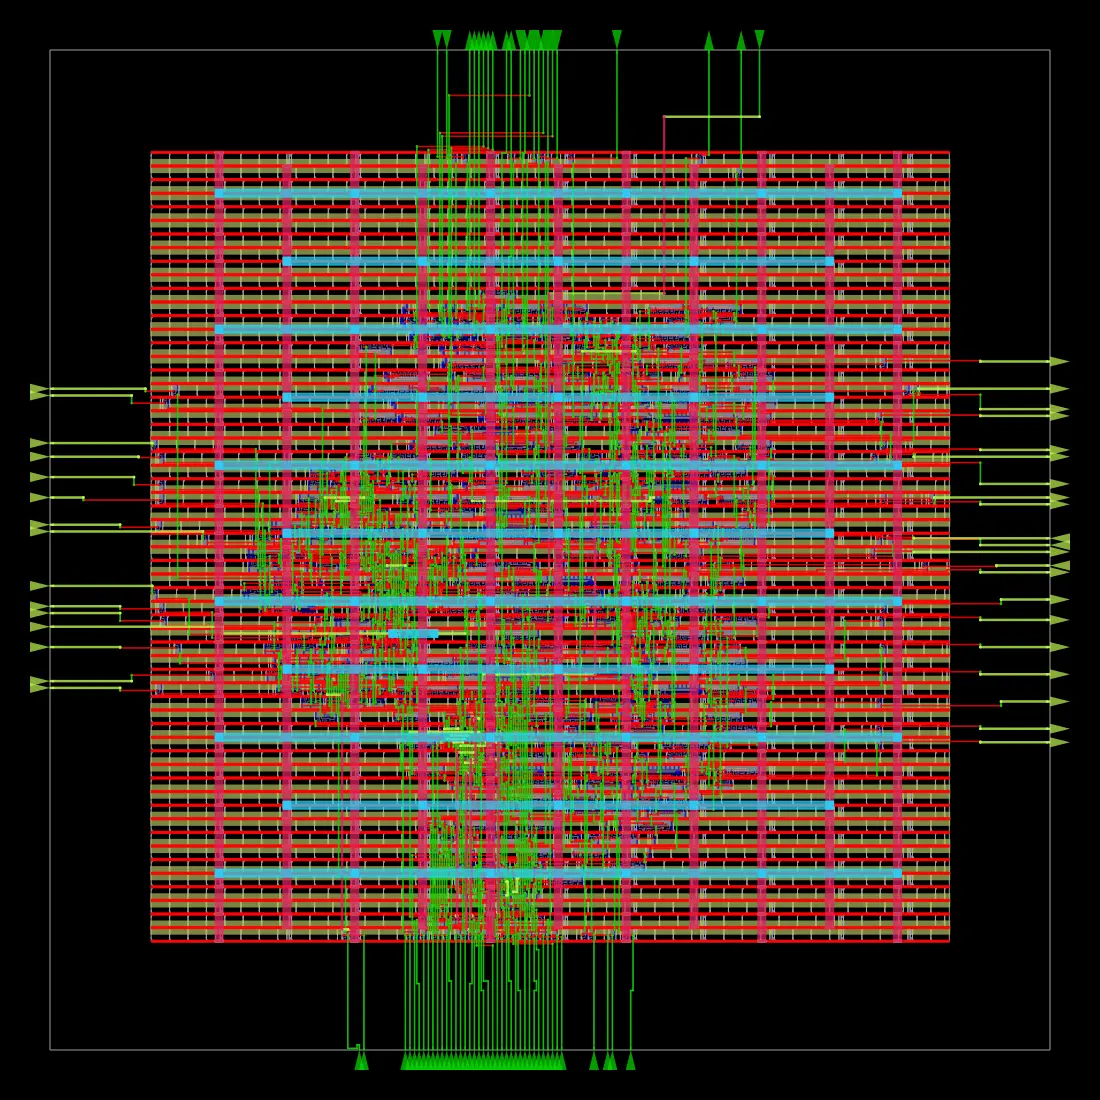
\includegraphics[width=\linewidth]{figures/vlsi/skag_w1_final_all.png}
\caption{SKAG-W1.}
\end{subfigure}\hfill
\begin{subfigure}[t]{0.32\textwidth}
\centering
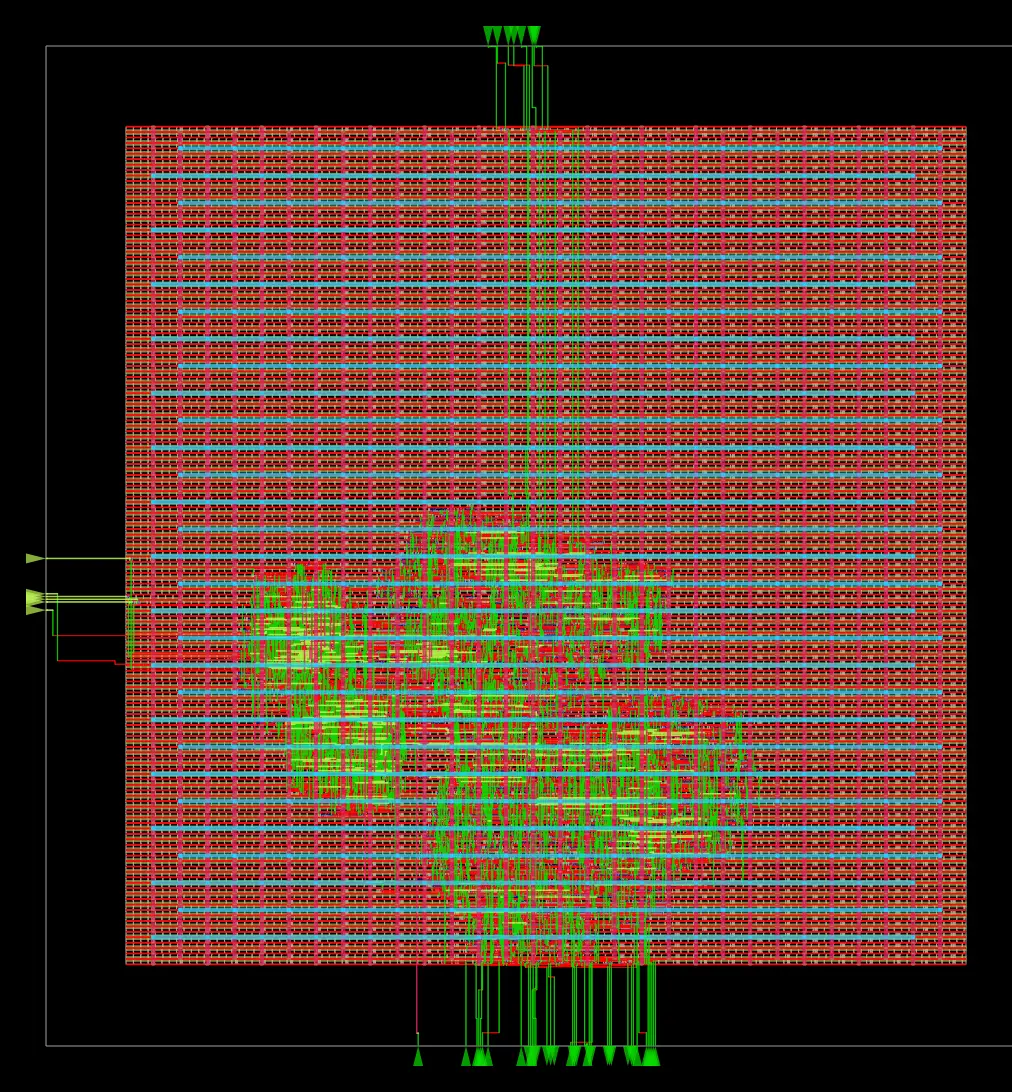
\includegraphics[width=\linewidth]{figures/vlsi/fdpe_v3_final_all.png}
\caption{LUT/interpolation kernel (FDPE-V3).}
\end{subfigure}\hfill
\begin{subfigure}[t]{0.32\textwidth}
\centering
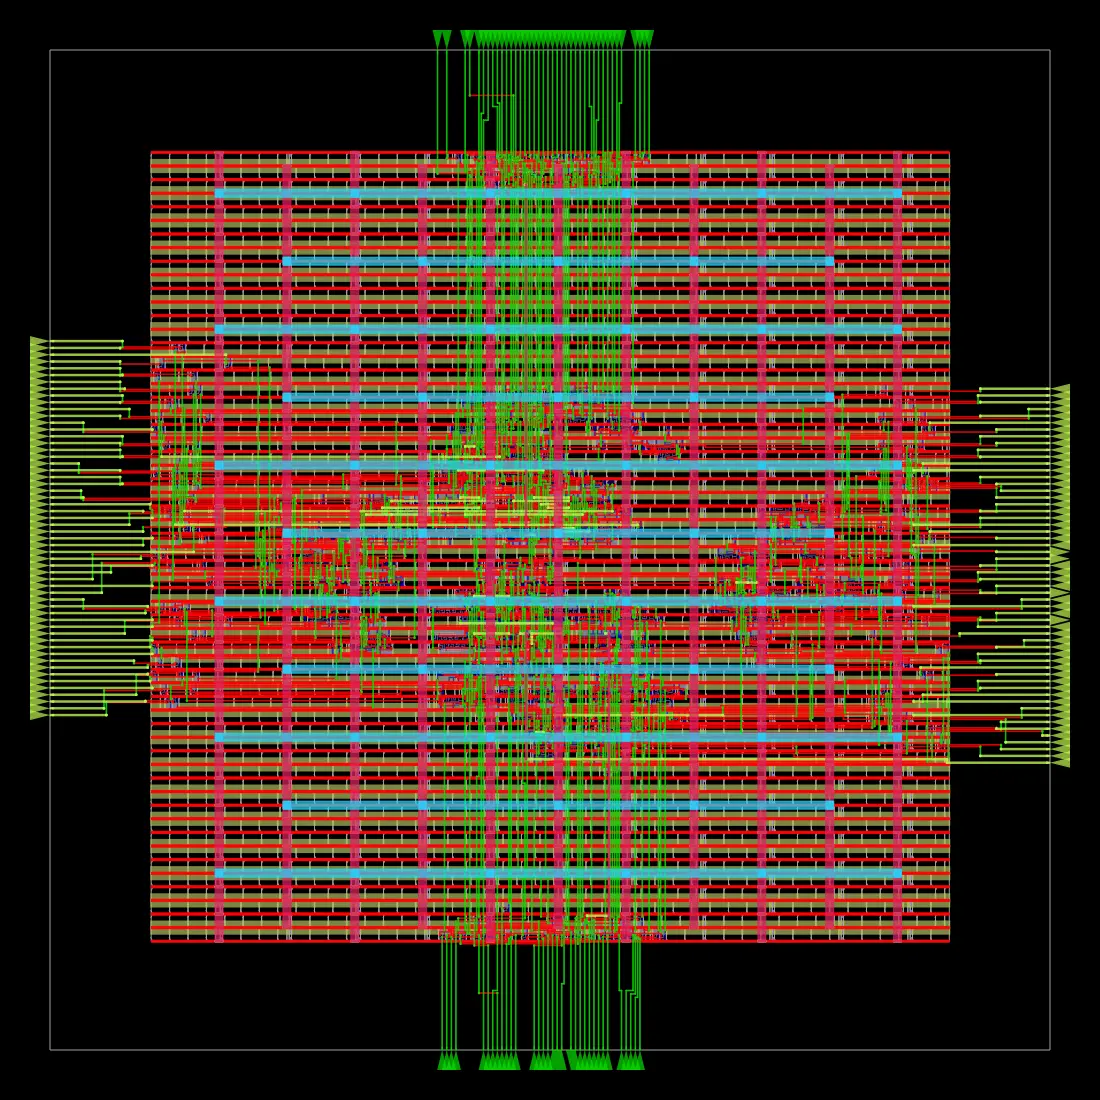
\includegraphics[width=\linewidth]{figures/vlsi/pareto_c0_final_all.png}
\caption{Pareto-C0.}
\end{subfigure}
\caption{Routed OpenROAD layouts for three isolated kernels. These views do not
represent an integrated \QFlow\ ASIC.}
\label{fig:vlsi-layouts}
\end{figure}

\begin{figure}[H]
\centering
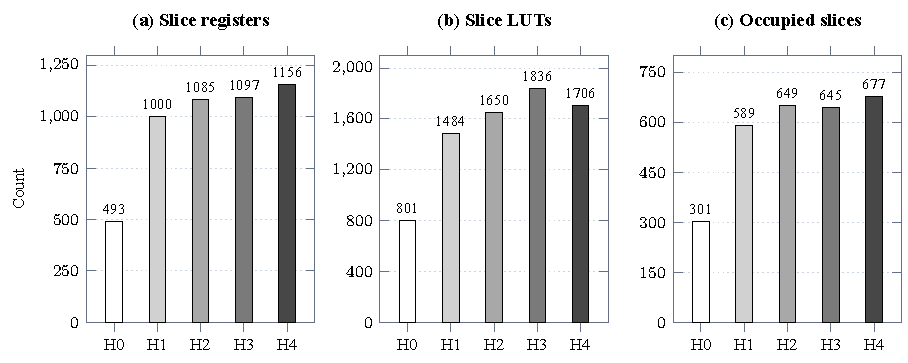
\includegraphics[width=\textwidth]{figures/new/resource_utilization_h0_h4.pdf}
\caption{Post-route FPGA resource utilization for the five independent
configurations. The aligned, zero-based panels report exact slice-register, slice-LUT,
and occupied-slice counts from Table~\ref{tab:resources}; grayscale shade identifies
H0 through H4 consistently in each panel. H4 mapped to fewer LUTs than H3 but used
more registers and occupied slices, so individual resource categories and physical
slice packing need not move in the same direction.}
\label{fig:resource_utilization}
\end{figure}

The flows generated routed reports and final artifacts for the separate kernels,
showing that selected functions can pass through an open-source physical-design
workflow. The areas must not be summed as a \QFlow\ chip area. The study does not
provide full-chip power, commercial DRC/LVS signoff, tapeout, or fabricated-silicon
performance.

\section{Threats to Validity}

\begin{itemize}
  \item The physical experiment used one FPGA board and device family.
  \item The physical corpus contained 84 rows per configuration and a bounded
  candidate set.
  \item The offline-learned policy was evaluated in a controlled research
  environment rather than across many independent unseen topologies.
  \item Replay rows may share structure, reducing the effective independence and
  power of route-quality tests.
  \item No matched CPU benchmark, activity-calibrated power measurement, or live
  KMS/SDN deployment was available.
  \item Configuration H4 performed inference only; online learning was not tested.
  \item Training used profile-dependent $\alpha$ coefficients and objective ratios,
  whereas the physical replay deployed only the ratio projection over supplied
  profile-independent path costs.
  \item The OpenROAD results concern isolated kernels and do not establish a
  complete ASIC implementation.
\end{itemize}

\section{Answers to the Research Questions}

\begin{table}[H]
\centering
\footnotesize
\caption{Answers to the research questions.}
\label{tab:rq-answers}
\begin{tabularx}{\textwidth}{@{}p{0.08\textwidth}X p{0.26\textwidth}@{}}
\toprule
\textbf{RQ} & \textbf{Answer} & \textbf{Evidence}\\
\midrule
RQ1 & All five independent configurations exceeded the 100~MHz post-route target. &
Table~\ref{tab:same-board-timing}\\
RQ2 & All 420 records and 3,780 checked fields matched exactly, with zero mismatch. &
Table~\ref{tab:physical-exactness}\\
RQ3 & Configurations H1--H4 required more logic and cycles than minimal configuration
H0; configuration H4 added small timing changes relative to H3. &
Tables~\ref{tab:resources} and \ref{tab:h4-h3-tradeoff}\\
RQ4 & Configuration H4 used all four profiles and the complete controller produced
45.455\% fewer transitions than configuration H3 on the replay. &
Table~\ref{tab:adaptation}\\
RQ5 & The held-out comparisons did not establish statistically significant
route-quality improvement. & Table~\ref{tab:pairwise-quality}\\
\bottomrule
\end{tabularx}
\end{table}

\section{Research-Hypothesis Outcomes}

\begin{table}[H]
\centering
\footnotesize
\caption{Mapping from research hypotheses to evidence and outcomes.}
\label{tab:hypothesis-outcomes}
\begin{tabularx}{\textwidth}{@{}p{0.12\textwidth}p{0.25\textwidth}p{0.18\textwidth}X@{}}
\toprule
\textbf{Hypothesis} & \textbf{Evidence} & \textbf{Outcome} &
\textbf{Interpretation}\\
\midrule
RH1 & Five post-route maximum-frequency reports & Supported & Every configuration
exceeded 100~MHz\\
RH2 & 3,780 field comparisons & Supported & Zero physical/reference mismatch\\
RH3 & 2.048~$\mu$s H4 latency and implementation metrics & Supported &
Microsecond-scale inference with measured resource/timing trade-offs\\
RH4 & 44 versus 24 transitions & Supported & Complete H4 policy-and-dwell controller
switched less on the common replay\\
RH5 & Paired CIs and $p$-values 0.2188 and 0.4531 & Not supported & Route-quality
superiority was not established\\
\bottomrule
\end{tabularx}
\end{table}

{\small\textbf{Chapter conclusion.} RH1--RH4 are supported; RH5 is not. The FPGA
evidence establishes exact, microsecond-scale adaptive behavior, but neither
route-quality superiority nor an integrated ASIC.\par}
